
\documentclass[12pt]{report}

\usepackage{setspace}
\onehalfspacing %doublespace %
\usepackage{amssymb,amsmath,amsthm}

\setlength{\intextsep}{1ex}

%\usepackage[dvips]{graphicx}
\usepackage{graphicx}
\include{epstopdf}
\renewcommand{\qedsymbol}{\rule{0.4em}{0.4em}}
\usepackage{tabularx}
\usepackage{multicol}
\usepackage[a4paper,bindingoffset=25mm,%
            left=0mm,right=15mm,top=15mm,bottom=15mm,%
            footskip=5mm]{geometry}

\usepackage{lipsum}  
%\usepackage{pstricks}
%\usepackage{pst-node}
%\usepackage{pst-blur}
\usepackage{tikz}
\usetikzlibrary{shapes.geometric, arrows}
\usepackage{xparse}
\usepackage{float}
\setlength{\intextsep}{1ex}
\usepackage[shortlabels]{enumitem}
\usepackage{multirow}
\usepackage[font={small}]{caption}
\usepackage{nameref}
\usepackage{wrapfig}
\usepackage[justification=centering]{caption}
\usepackage{caption,subcaption}
\usepackage[toc,page]{appendix}


\setlength{\parskip}{10pt}
\setlength{\parindent}{0pt}

\renewcommand{\bibname}{References}


\setlength\parindent{0pt}
\setlength{\unitlength}{1cm} 


\begin{document}

\begin{titlepage}
\centering

\begin{figure}[H]
\centering

\includegraphics[width=0.4\textwidth]{maklogo.png}%
\end{figure}


\textsc{}

\vspace{\stretch{0.1}}

{\huge \textsc{A Vehicle to Vehicle Communication Model for Collision Avoidance in Autonomous Cars}  \\}
\rule{3in}{0.4pt}

\vspace{\stretch{0.4}}

{\Large\textbf{Aanyu Deborah Oduman}	 \\}
Student ID: 16/U/2070\\ \vspace{2cm}
{\large \textbf{Department of Electrical and Computer Engineering} \\
School of Engineering \\
College of Engineering, Design, Art and Technology}



\vspace{\stretch{0.3}}

{
Supervisor: \textbf{Dr. Edwin Mugume}    \\
Co-supervisor: \textbf{Mr. Paul Bogere} }

\vspace*{\stretch{0.2}}

% Add date in desired format
December 04, 2020


\vspace*{\stretch{0.2}}
% Add the statement of what the report represents
{
A Report submitted in partial fulfillment of the requirements for the \\ \textbf{ Degree of Bachelor of Science in Computer Engineering} \\ at Makerere University. }


\end{titlepage}
\pagenumbering{roman}


%\maketitle
				
%\beforeabstract %\input{abstract} 


\section*{Declaration}

I, \textbf {Aanyu Deborah Oduman}, solemnly and sincerely declare this report compiled, written and designed by me. I have not submitted a copy to any other institute for any academic certificate or award. The information in this report is based on my work and experience as I undertook my final year project. Any other information not availed by me is well referenced.

\textbf{I HAVE ABIDED BY THE MAKERERE UNIVERSITY ACADEMIC INTEGRITY POLICY ON THIS PROJECT.}

\bigskip

\begin{multicols}{2}
	\textbf{Signature:} Aanyu Deborah Oduman 
	
	\textbf{Date: } 04-12-2020
\end{multicols}


\newpage



\section*{Approval}

This dissertation entitled "A Vehicle to Vehicle Communication Model for Collision Avoidance in Autonomous Cars" has been done under our supervision and has been submitted to the College of Engineering, Design, Art, and Technology, Makerere University for examination with our approval as the candidate supervisors.


\vspace{2cm}

Signature \rule{2in}{0.4pt}\hspace{1cm} Date \rule{2in}{0.4pt} \\
\textbf{Dr. Edwin Mugume} \\
Main Supervisor\\

\vspace{1cm}

Signature \rule{2in}{0.4pt}\hspace{1cm} Date \rule{2in}{0.4pt} \\
\textbf{Dr. Andrew Katumba } \\
Co-Supervisor


\newpage

\section*{Dedication}

\begin{center}
I dedicate this report to my family that has tirelessly supported me throughout my education life, to this level. I pray the Almighty God richly blesses you. I also dedicate it to those that genuinely care about making the world a better place by generously using that which God has given to them.
\end{center}




\newpage

\section*{Acknowledgements}

I am grateful for the life, good health and protection the Almighty God granted me during the course of this final year project. I am also very grateful for my family and dear friends for the unwavering support and encouragement especially during these unpredictable times. 

I am thankful to my project partner, Isanga Nadia Hanifa for the teamwork, support, and commitment towards achieving our goal for this project.

I would like to thank Dr. Edwin Mugume in a special way for the immense support, encouragement and the commitment of his time and knowledge to ensure that we achieved the set objectives for this project. May the Almighty God richly bless you.

I would also like to thank my co-supervisor, Mr. Paul Bogere for the guidance, advice and support  during this project.





\newpage



\section*{Abstract}

This paper proposes a Vehicle to Vehicle communication-based model for collision avoidance by analysing the various parameters shared during communication and using the results of this analysis to provide warning signals to the autonomous cars to avoid collision. The proposed collision avoidance algorithms greatly benefit from the information exchange between the vehicles that are inside the Vehicular Ad-hoc network to calculate safe accelerations, distances, and velocities that the vehicles would later take on to guarantee the avoidance of collision. Simulations were done for three scenarios namely; Blind Spot, Intersection Movement Assist and Forward Collision all of which were implemented using MATLAB. The results show that the proposed collision avoidance system makes a composite analysis of the collision risk and then takes the necessary action to avoid the collision.

\newpage

\tableofcontents

\newpage

\listoffigures

\newpage

\listoftables

\newpage



\section*{List of Abbreviations}

\begin{tabular}{p{3cm} l}
	3G &Third Generation Mobile Network\\
	4G &Fourth Generation Mobile Network\\
	5G &Fifth Generation Mobile Network\\
	BSW &Blind Spot Warning\\
	DSRC &Dedicated Short Range Communications\\
	DTC &Distance to Collision\\
	FCW &Forward Collision Warning\\
	GPS &Global Positioning System\\
	I2V & Infrastructure to Vehicle Communication\\
	IMA &Intersection Movement Assist\\
	ISM &Industrial, Scientific and Medical\\
	ITS &Intelligent Transport Systems\\
	LTE &Long Term Evolution\\
	MANET &Mobile Ad hoc Network\\
	NHTSA &National Highway Traffic and Safety Administration\\
	OBU &On Board Unit\\	
	V21 & Vehicle to infrastructure Communication\\
	V2N & Vehicle to Network Communication\\
	V2P & Vehice to Person Communication\\
	V2V	& Vehicle to Vehicle Communication\\
	V2X & Vehicle to Everything Communication\\
	VANET &Vehicular Ad Hoc Network\\
	WHO &World Health Organisation\\
	WiFi &Wireless Fidelity\\
	
	

\end{tabular}


\newpage

\section*{Symbols and Notations}

\begin{tabular}{p{3cm} l}
	$\mu$						& coefficient of friction \\
	$a$ 						& acceleration \\
	$a_{fv}$					& acceleration of the following vehicle \\
	$a_{lv}$					& acceleration of the leading vehicle \\
	$D_w$						& distance warning \\
	$f$ 						& frictional coefficient based on speed \\
	$g$							& acceleration due to gravity \\
	$G$							& universal gravitational constant \\
	$m$							& mass \\
	$s$							& distance covered by the car \\
	$t$							& time \\
	$t_d$						& delay time/ brake time \\
	$t_{GPS}$					& GPS update period \\
	$t_w$						& time to warning \\
	$U_a$						& initial velocity of Car A \\
	$U_b$						& initial velocity of Car B \\
	$U_r$						& relative velocity between Car A and B \\
	$u$							& initial velocity \\
	$v$							& final velocity \\


	
	
\end{tabular}




\chapter{INTRODUCTION}

\section{Background}

World wide, the key facts are approximately 1.35 million people die each year as a result of road traffic crashes.
The 2030 Agenda for Sustainable Development has set an ambitious target of halving the global number of deaths and injuries from road traffic crashes by 2020.
Road traffic crashes cost most countries 3\% of their gross domestic product \cite{traffic}.
More than half of all road traffic deaths are among vulnerable road users: pedestrians, cyclists, and motorcyclists.
93\% of the world's fatalities on the roads occur in low- and middle-income countries, even though these countries have approximately 60\% of the world's vehicles \cite{traffic}.
 
Road traffic injuries are among the leading causes of death and life-long disability globally. The World Health Organization (WHO) reports that about 1.24 million people die annually on the world’s roads, with 20–50 million sustaining non-fatal injuries \cite{systematic}. Globally, road traffic injuries are reported as the leading cause of death among young people aged 15–29 years and are among the top three causes of mortality among people aged 15–44 years \cite{systematic}.

In Africa, the number of road traffic injuries and deaths have been increasing over the last three decades. According to the 2015 Global status report on road safety, the WHO African Region had the highest rate of fatalities from road traffic injuries worldwide at 26.6 per 100,000 population \cite{systematic}.

In Uganda, the accident severity index is 24 people killed per 100 road crashes \cite{road}]. On average, Uganda loses 10 people per day in road traffic crashes, this is the highest in East Africa. These crashes cost an overall annual cost estimated at approximately UGX 4.4 trillion (\$ 1.2 billion), representing 5\% of Uganda’s gross domestic product (GDP) \cite{road}. Uganda’s road infrastructure is generally unsafe. Most of the roads are single carriageway without a median, many with steep shoulders and with few opportunities for overtaking, resulting in many head-on collisions.

This high number of fatalities from road crashes can be attributed to factors such as reckless driving, over speeding, drunk-driving or alcoholism, inadequate road traffic signs, incompetent 
\pagenumbering{arabic}
drivers or riders, among other factors.

A number of measures have been put forward to try to curb the high number of deaths from road accidents. Some of these include:
	\begin{itemize}
		\item The introduction of computerized driving permits:The security features of the computerized driving permit have been enhanced to conform to the current international standards to minimise forgeries [4].
		\item Launching of traffic operations such as "Fika Salama". Fika Salama is an operation that was initiated by Uganda police in collaboration with Uganda National Roads Authority and Ministry of Works and Transport and several health facilities in response to the increased road accidents that were happening on Kampala- Masaka road \cite{fikasalama} This was to raise awareness about road safety following harrowing road accidents that had been occuring in the past six months.
		\item Licensing and inspection of driving schools. This is to endeavour that driving schools and teachers are teaching people to drive using the proper methods are are doing so, under the government recommended standards.
		\item The Road Crash Data System project; the recording of road crashes or accidents had gone digital under the digital road crash data system. This was done to collect data on the number of accidents occurring on Ugandan roads and to use this data to find sustainable solutions to the issue of road safety \cite{road}.
	\end{itemize}

\section{Problem Statement}
Despite all the above preventive measures that have been put forward to try to tackle the issue of road safety, the number of road accidents still remains alarmingly high. Therefore, there is need to enable vehicles communicate with each other reliably, and distribute some of the decision making to a smarter, more intelligent system that will use the information obtained the exchange of messages to detect possible collisions and automatically take action to avoid them.

Vehicle to Vehicle (V2V) communication allows cars to communicate
with each other in an effort to warn drivers about potential accidents and prevent crashes.
The National Highway Safety Administration (NHTSA), believes V2V
technology has the potential to reduce the number of multi-vehicle crashes by 82\% \cite{talk}.


\section{Aims and Objectives}

The main aim of the research project was to design a communication-based collision avoidance model for
autonomous cars.

\subsubsection{The specific objectives of the research were:}

\begin{itemize}[topsep=0pt]

\item To understand some of the main traffic scenarios around which many road accidents occur - junctions, bends, lane changes, etc
\item To simulate an algorithm that will use the (real time) data provided to issue the appropriate collision avoidance warning to the vehicle.
\item To design scenarios in which the car driver is warned of the possible collision and how the autonomous car will take action to avoid this
collision. 

\end{itemize}


\section{Contributions of the Project}

The following major contributions have been accomplished during the course of this research:

\begin{enumerate}[topsep=0pt]

\item Developed communication models and designed algorithms for the common traffic scenarios around which accidents usually occur namely; intersections, blind spots, and forward collision on straight roads. 

\item Performed simulations in MATLAB of the algorithms for each of the scenarios mentioned above, providing values from real life data.

\item Proposed collision avoidance models whereby the car is faced with an incoming collision and we observe the vehicle making a decision  basing on the information that it has been provided, and takes action to avoid the collision.

\end{enumerate}






\section{Organization of the Report}

This report has five chapters. 

Chapter one is the introduction to the entire project. It gives a background on what was considered for this research, the problem statement that was formulated, as well as the aims and objectives that this project is targeted to accomplish.

Chapter two gives the literature review on the major concepts that were often used throughout the course of the project. The concepts are described in greater detail to provide a proper basis for the implementation of the project.

Chapter three then describes the methods and tools that were used during the course of implementation/ simulation of the project targeted toward achieving the said objectives in chapter one.

Chapter four contains the results and analysis that was achieved as a result of using the methodology in chapter three. The results obtained are mostly from simulations in MATLAB software.

Chapter five concludes the project. It reveals whether our results in chapter four met our said objectives in chapter one. Challenges faced during the course of the project are also highlighted here, and recommendations proposed could possibly overcome the aforementioned challenges. The chapter also mentions potential future areas of research in the topic of vehicle to vehicle communication.




\chapter{LITERATURE REVIEW}
% Usually Literature Review

\section{Introduction}

The background information provided in this chapter forms the basis for this project. This section highlights the various communication technologies that were considered for this V2V project. Vehicular Ad hoc networks are also looked at in detail as well as the various modes of V2V communication.


\section{Wireless Communication Technologies for Vehicles}
Several existing wireless technologies can support vehicle communications. Short-range radios include Bluetooth, Wi-Fi, and dedicated short-range communications (DSRC). Long-range radios include cellular networks, satellite services, and digital radio broadcast networks.

	\subsection{Bluetooth}
	Bluetooth operates in an unlicensed 2.4 GHz industrial,	scientific, and medical (ISM) frequency band. Bluetooth is increasingly used to pair mobile phones to vehicles. Bluetooth also enables a vehicle to use the driver’s or a passenger’s
	mobile phone to communicate with the outside world to support a wide range of telematics applications such as making emergency calls when the driver loses ability to do so in an accident, downloading digital maps, infotainment, travel information among others. Bluetooth can also been used for some V2I communications
	when the vehicle is stationary or moving at very low speeds. These include, for example, allowing a vehicle to communicate with parking lot payment applications at a parking lot entrance. However, bluetooth’s limited communication range and high latency precludes its ability to support vehicle safety communications.
	
	\subsection{WiFi}
	Wi-Fi networks, defined in the Institute of Electrical and Electronics Engineers (IEEE) 802.11 standards, can support V2V local broadcasts through their native ad hoc broadcast capabilities. However, modifications to the standards \cite{protocols}.
	are necessary to reduce latency and achieve more reliable communications at high speeds in order to support vehicle safety communications. Wi-Fi networks can also support other forms of vehicle communications in their infrastructure mode. However, Wi-Fi hotspots have sparse coverage today and
	moving from one hotspot to another generally requires reconnection to the network. This could be tolerated by some non-safety vehicle applications. So far, IEEE 802.11 technology is the closest to meeting most requirements
	of hard safety applications leading to the development of DSRC radio technology and standards. DSRC is essentially Wi-Fi in its ad hoc mode adapted	to support communications among vehicles moving at high speeds.
	
	\subsection{Cellular}
		\subsubsection{3G}
		Third - generation (3G) cellular networks offer communication latencies in
		the range of hundreds of milliseconds, thus meeting the requirements of some
		hard and soft safety applications. However, current 3G networks lack effective ways to support V2V local broadcasts, which are essential to most hard safety
		applications \cite{protocols}. Furthermore, sharing bandwidth with voice communications
		could cause unpredictable delays and could also overload the cellular system.
		Addressing this issue by using a separate cellular system for vehicle communications
		could be costly. Also, the long call setup latencies can introduce
		excessive delays for vehicle safety applications.
		
		\subsubsection{4G}
		The predominate fourth generation (4G) cellular network technology,	Long - Term Evolution (LTE), offers significantly lower communication delay, higher capacity, and enhanced broadcasting capabilities compared with 3G cellular networks. LTE can also support very small radio cells. These small cells can be used to deliver even higher capacity and lower delay at hot spots such as
		homes, office building complexes, densely populated areas, and crowded road intersections. Therefore, LTE can support time-critical vehicle applications, including selected I2V local broadcast and V2V safety applications \cite{protocols}.
		
		\subsection{5G}
		5G is designed to deliver peak data rates of up to 20 Gbps \cite{qualcomm}. 5G will investigate the issues within the technologies mentioned above and will also address the performance criteria for low latency, high speed, enhanced reliability, peak throughput per connection, system spectral efficiency, connection capacity density, and low power consumption. With all these desirable qualities, 5G  will enable vehicles to interact in real time with their environment so as to increase road safety, traffic efficiency, and energy savings \cite{protocols}.

\section{Safety Applications Addressed by V2V}
Potential V2V safety applications include safety warnings for drivers, such as: Emergency electronic brake lights warning, Forward  collision warning, Intersection movement assist warning, Blind spot warning, Lane change warning, Do not pass warning, Control Loss Warning, Bus Driver Warning – vehicle making a right turn in front of a bus among others.

\begin{figure}[!hb]
	%\centerline [scale=0.7]{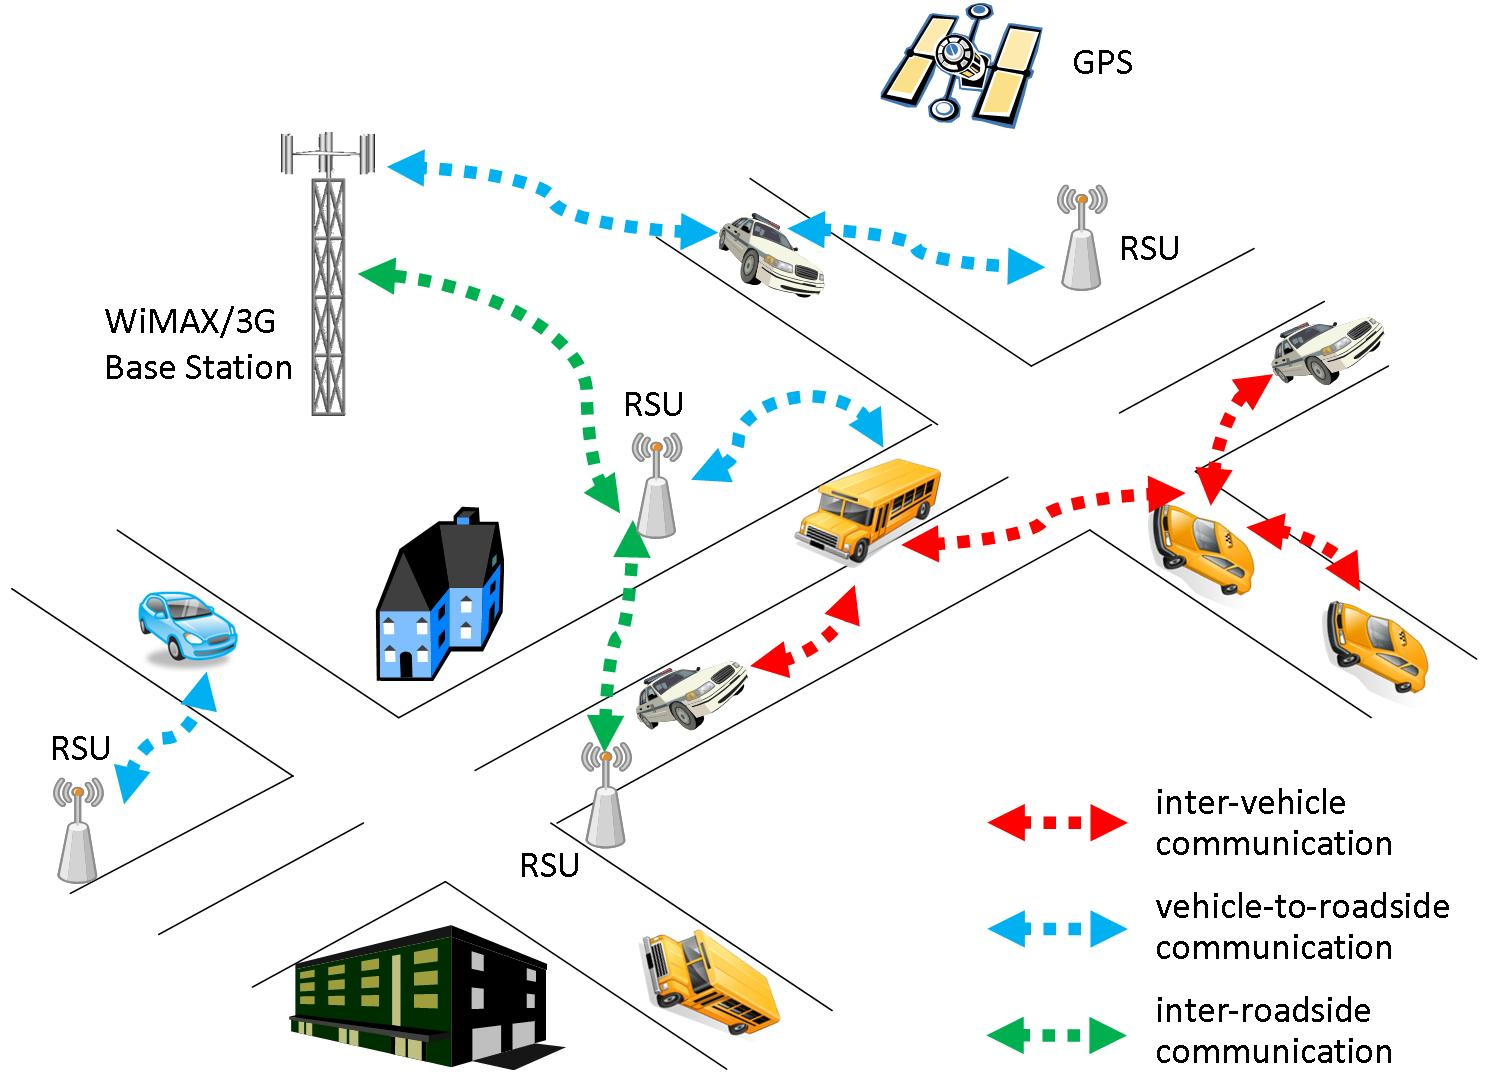
\includegraphics{VANET.png}}
	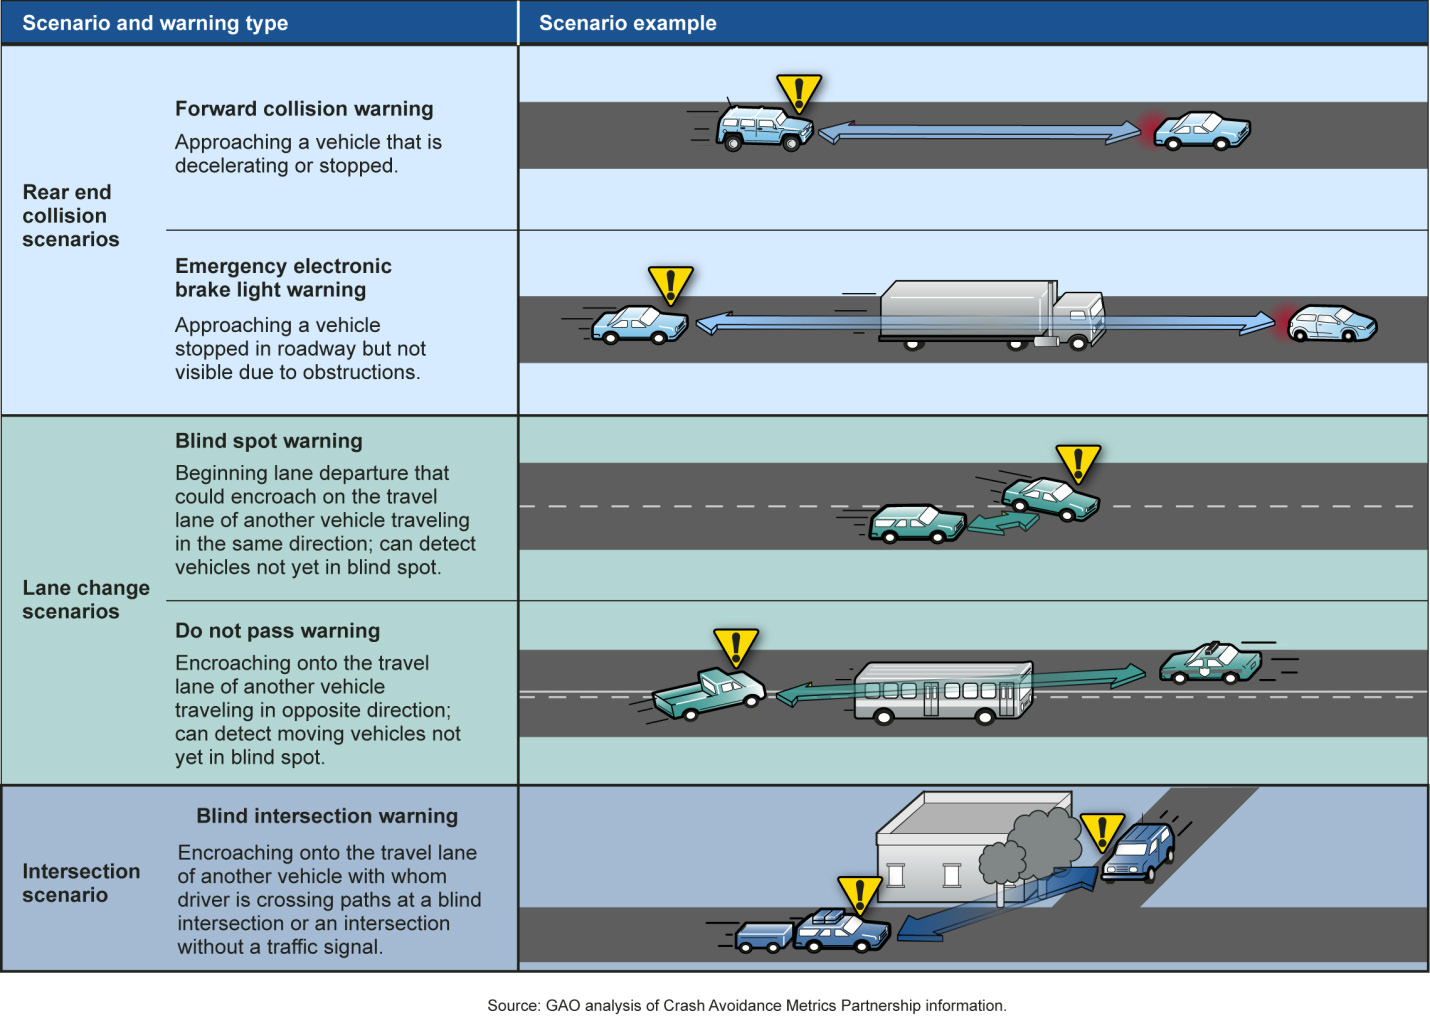
\includegraphics[width=1.0\textwidth]{warnings.png}
	\caption{Examples of safety warnings addressed by V2V and their descriptions \cite{readiness}}
	\label{fig}
\end{figure}

\section{Vehicular Ad Hoc Networks (VANETs)}
Vehicular Ad-Hoc Networks  allow Dedicated Short Range Communications of vehicles in the 5.9 GHz band, through the IEEE 802.11p standard. They support Intelligent Transport Systems  with both (V2V) and (V2I) communications for applications in both near and far environment \cite{protocols}. 
Vehicular Ad hoc Networks are created by applying the principles of mobile ad hoc networks and are a sub-case of Mobile Ad hoc Networks. 
However, they differ from MANETs since their end-to-end connectivity is not guaranteed and the vehicles (i.e. the nodes of the network) are highly mobile. Moreover, they can scale up to very large networks, but the probability that they split into parts is high \cite{protocols}. VANETs use any wireless communication technology to generate the networks enhancing Vehicle-to-Vehicle communication, as well as  vehicle-to infrastructure communication. 

VANETs are at high risk of partitioning, as their topology changes quickly. This means that there will be possibly a lot of disconnections during those alterations in their network structure. This characteristic makes the designing of an efficient solution to disseminate data in a particular way between vehicles a very difficult challenge in the area of V2V communications \cite{protocols}. 

\begin{figure}[!hb]
	%\centerline [scale=0.7]{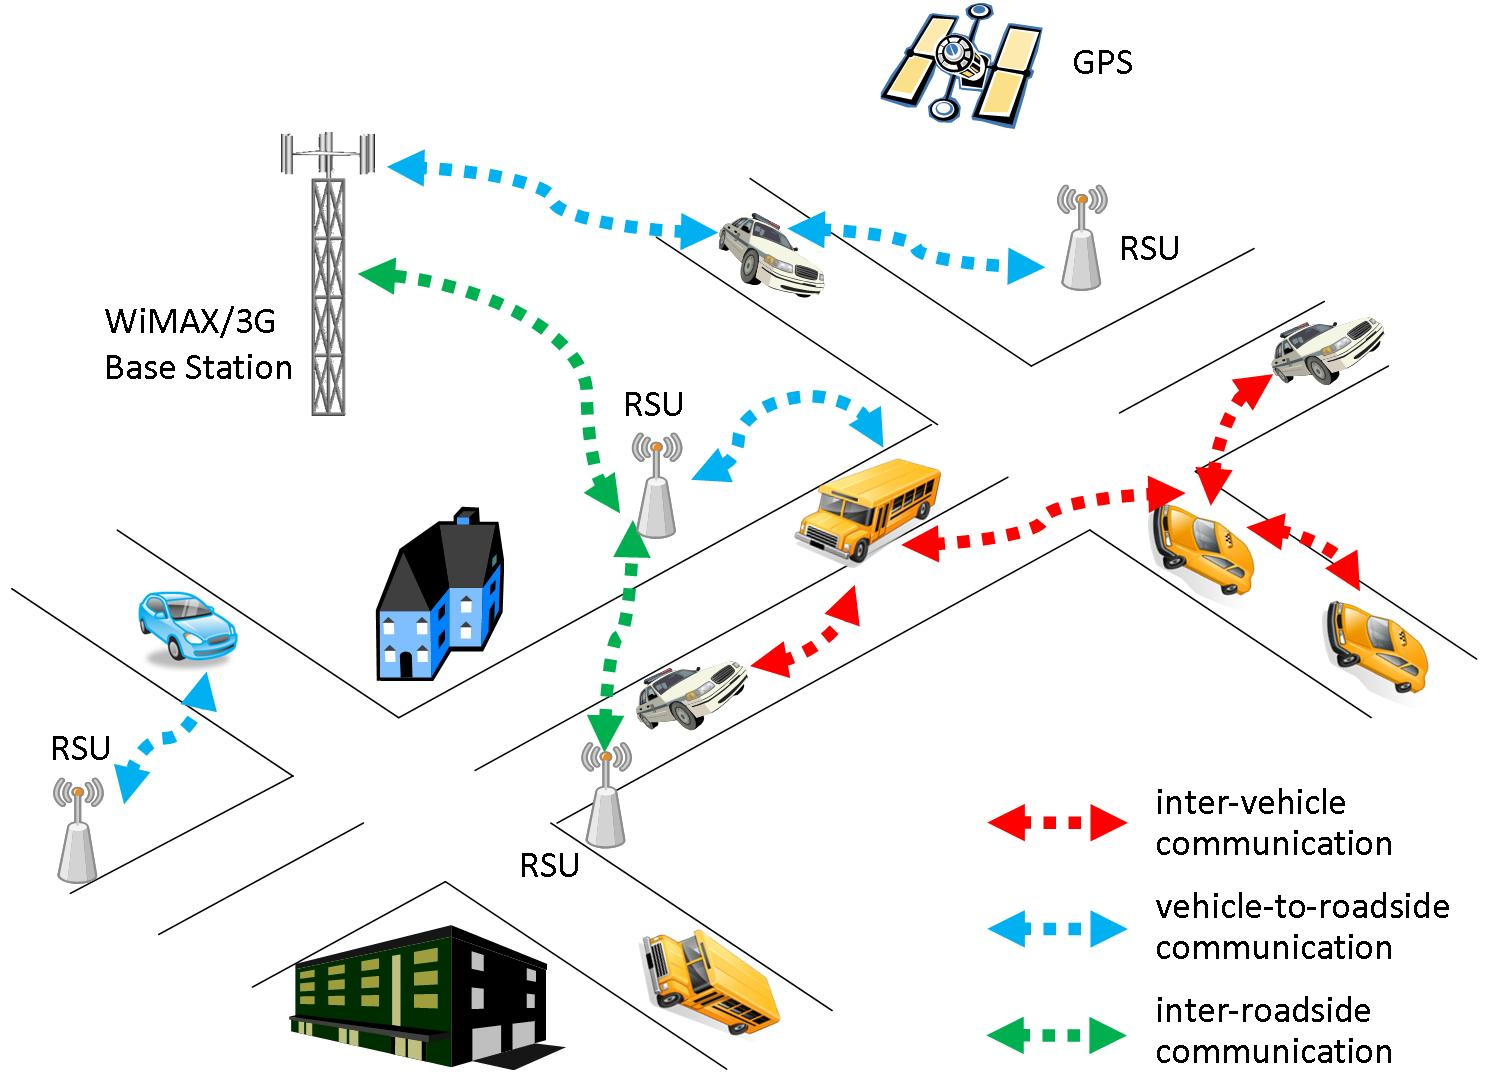
\includegraphics{VANET.png}}
	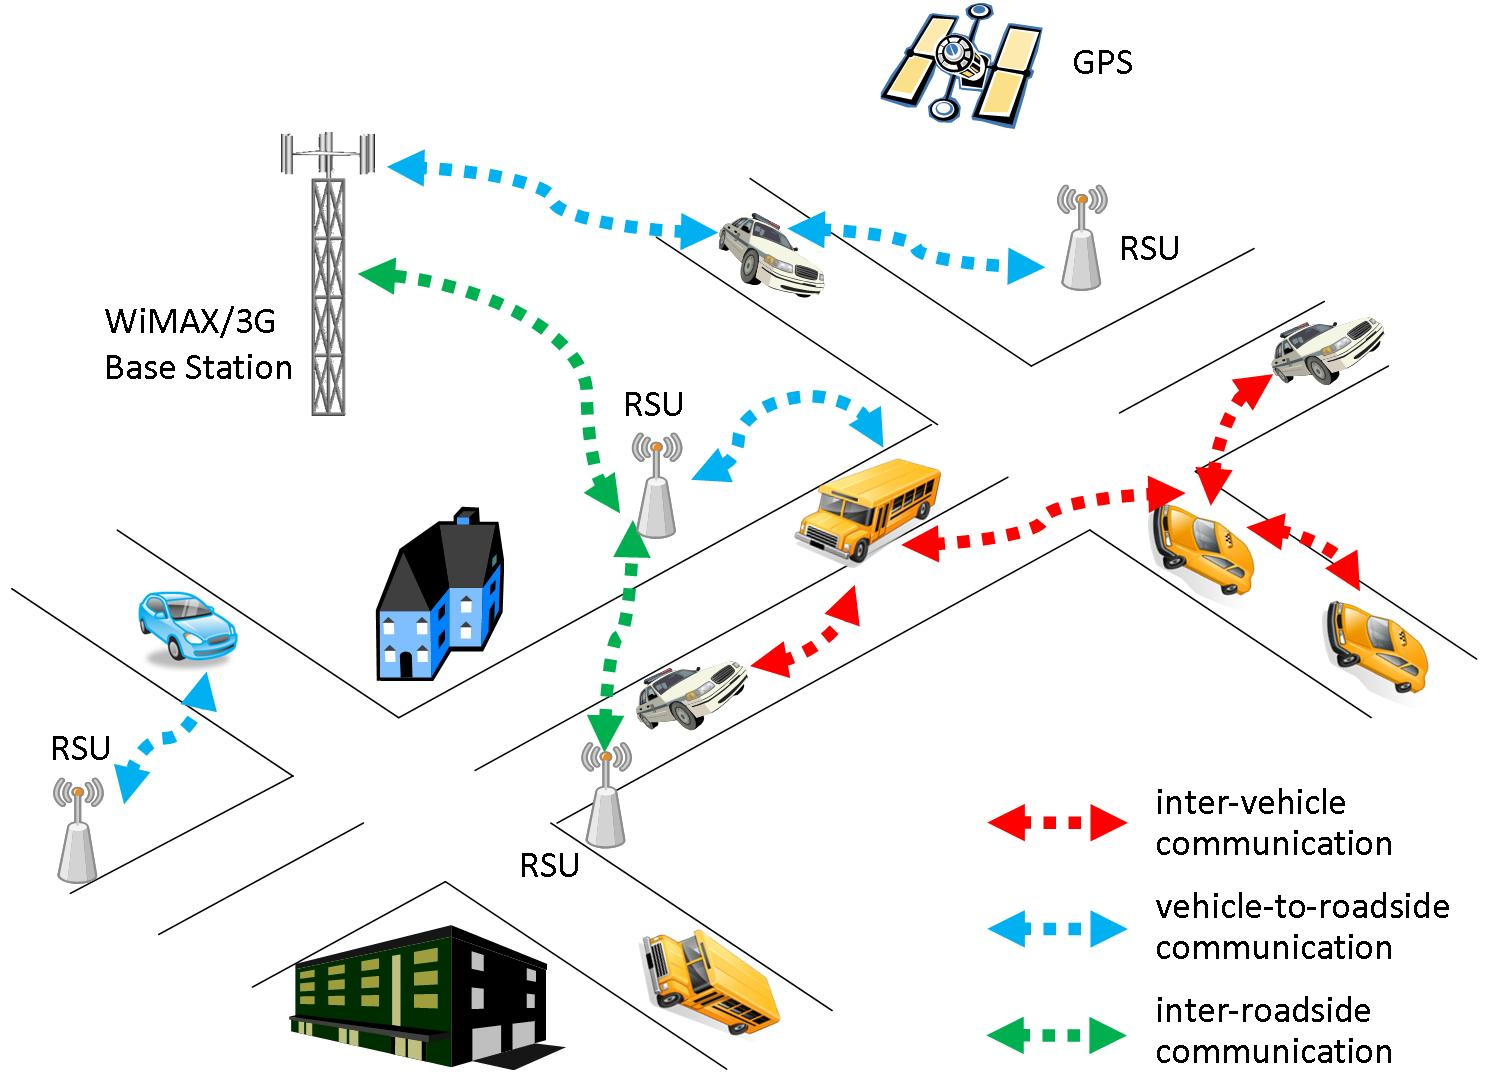
\includegraphics[width=0.9\textwidth]{VANET.jpg}
	\caption{Illustration of a Vehicular Ad Hoc Network \cite{readiness}}
	\label{fig}
\end{figure}

\section{Vehicle-to-Vehicle Communication}
Several vehicle communication modes can be envisioned as illustrated in the figure below. 
a) Vehicles can directly exchange safety messages through local broadcasts. b) These messages can be further relayed across multiple hops to reach other vehicles not within the source vehicle’s communication range. c) A roadside infrastructure network can broadcast messages to vehicles. d) Vehicles can communicate with application servers or e) communicate with other vehicles through the infrastructure network \cite{protocols}.

\begin{figure}[!hb]
	\centerline{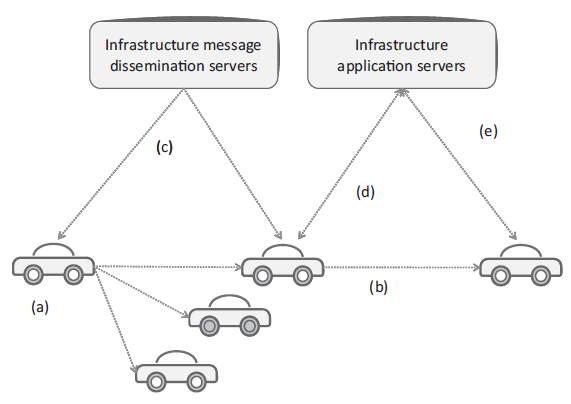
\includegraphics{v2v.png}}
	\caption{Vehicle safety communication modes \cite{protocols}. }
	\label{fig}
\end{figure}

(a) V2V local broadcast; (b) V2V multi-hop forwarding; (c) I2V local broadcast; (d) V2I bidirectional communications; (e) indirect V2V

	\subsection{ Vehicle-to-Vehicle Local Broadcast}
	With Vehicle-to-Vehicle local broadcast, a vehicle sends messages to all other vehicles within its communication range. These messages are not further relayed by other vehicles. This communication mode serves as the foundation for cooperative vehicle safety applications aimed at collision avoidance. For
	example, vehicles can use V2V local broadcast to inform neighbouring cars of each other’s current position, heading, and speed. When a vehicle broadcasts a safety message, it typically does not know whether there are other vehicles nearby. It is generally difficult for a vehicle to know the network addresses of other vehicles because the set of neighbouring vehicles changes frequently. For this reason, short-range radios with native broadcasting capabilities are natural ways to support this communication mode \cite{protocols}.
	
	\subsection{V2V Multi-hop Message Dissemination}
	With V2V multi-hop message dissemination, messages from one vehicle are relayed by other vehicles to reach vehicles that are not inside the source vehicle’s communication range. When the number of hops is very low, this communication mode can be used to support hard safety applications. V2V multi-hop message dissemination could also be used for soft safety purposes such as the distribution of hazardous road and traffic information.
	A fundamental issue in this design is how to balance performance and overheads. Important performance metrics include message dissemination delay and message delivery rate. Main overheads include the number of messages to be transmitted to implement
	a dissemination strategy, the amount of processing on each vehicle, and the implementation complexity.
	A second fundamental issue is that the vehicles may not always form a connected V2V network. Message dissemination needs to work despite random temporary network partitions \cite{protocols}.
	
	\subsection{Infrastructure to Vehicle Local Broadcast}
	With Infrastructure to Vehicle local broadcast, vehicles receive local broadcasts from the roadside infrastructure. It can be used to send: traffic controller signal phase and timing information,  dangerous road condition information, security credentials, and service advertisements
	I2V local broadcast can be implemented through short - range radio transceivers deployed along the roadside. It can also be implemented using cellular, satellite, or digital radio broadcast services to reach all the vehicles in a large geographical region. Satellite and digital radio broadcast services are widely
	available on vehicles today. They are commonly used to deliver real - time traffic and road conditions information to drivers and navigation devices \cite{protocols}.
	
	\subsection{Vehicle- to- Infrastructure Bi-directional Communications}
	Many mobility and convenience applications require the V2I bidirectional communications mode. Examples include navigation, internet access for browsing or e-mail, electronic transactions for purchasing	goods or services, and media download. Another important use is for vehicles to communicate with security credential
	management systems. V2I communications can also be used to “broadcast”	messages from a vehicle to other vehicles through infrastructure applications	servers.
	V2I communications can be supported using long-range or short-range radios. Short-range radio networks deployed along roadsides, homes, or in public hotspots such as parking lots and vehicle service centres can be used by vehicles to access infrastructure-based services \cite{protocols}.
	



\section{Summary}
Chapter two summarized the theory/literature review of the various communication technologies that were considered for this V2V project, vehicular Ad hoc networks and the various modes of V2V communication.



\chapter{METHODOLOGY}

\section{Introduction}

This chapter describes the active processes that were carried out in achieving the project objectives are described. 

\section{Project Process Flow}

\tikzstyle{startstop} = [rectangle, rounded corners, minimum width=3cm, minimum height=1cm,text centered, text width=15cm, draw=black]
\tikzstyle{process} = [rectangle, minimum width=3cm, minimum height=1cm, text centered, draw=black, fill=orange!30]
\tikzstyle{decision} = [diamond, minimum width=3cm, minimum height=1cm, text centered, draw=black, fill=green!30]
\tikzstyle{arrow} = [thick,->,>=stealth]

\begin{tikzpicture}[node distance=2cm]
	\node (start) [startstop] {Use Newton’s laws of motion to model the Forward Collision, Blind spot, and Intersection Movement Assist scenarios.
	};
	\node (start2) [startstop, below of=start] {Propose a traffic inter vehicle communication collision algorithm to prevent collisions for the three scenarios.
	};
	\node (start3) [startstop, below of=start2] {Simulate the algorithms in MATLAB software and use field values from all scenarios to observe how the collision will be avoided.
	};
	\node (start4) [startstop, below of=start3] {Propose a VANET based communication infrastructure through which the vehicles will be able to communicate with each other
	};
	\draw [arrow] (start) -- (start2);
	\draw [arrow] (start2) -- (start3);
	\draw [arrow] (start3) -- (start4);
\end{tikzpicture}

\section{Tools Used}
	\subsection{MATLAB}
	This is a multi-paradigm software that combines a desktop environment tuned for iterative analysis and design processes with a programming language that expresses matrix and array mathematics directly.
	
	\subsection{Microsoft Visio}
	Microsoft Visio is a diagramming and vector graphics application and is part of the Microsoft Office family. This tool was used for designing the communication infrastructure for each of collision scenarios.
	
\section{Forward Collision Warning}
A forward collision warning (FCW) system is an advanced safety technology that monitors a vehicle's speed, the speed of the vehicle in front of it, and the distance between the vehicles. If vehicles get too close due to the speed of the rear vehicle, the FCW system will warn that driver of an impending crash.

	\begin{figure}[!hb]
		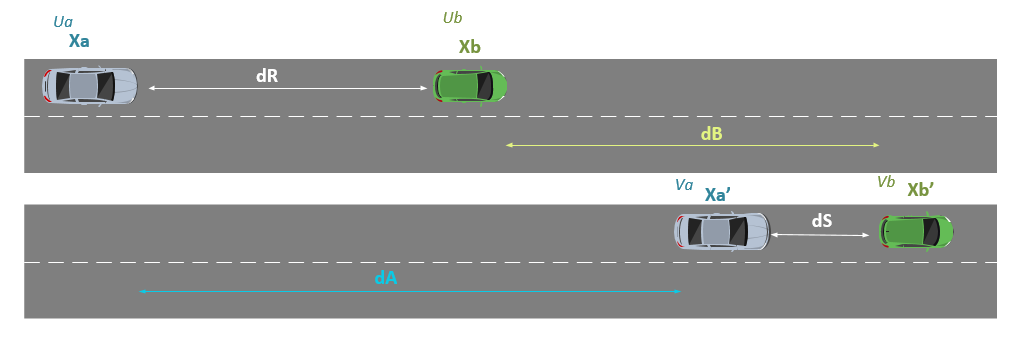
\includegraphics[width=1.0\textwidth]{forwardcollision.png}
		\caption{A forward collision scenario with parameters}
		\label{fig}
	\end{figure}

In the above figure, two cars can be observed trailing each other on a straight road. Both cars have different velocities as indicated in the figure. Car A (blue) moves from the point $X_a$ to the $X_a$’. Car A (green) moves from the point $X_b$ to the point $X_b$’. $d_A$ is thus the distance moved by Car A while $d_B$ is the distance moved by Car B.

\begin{figure}[!h]
	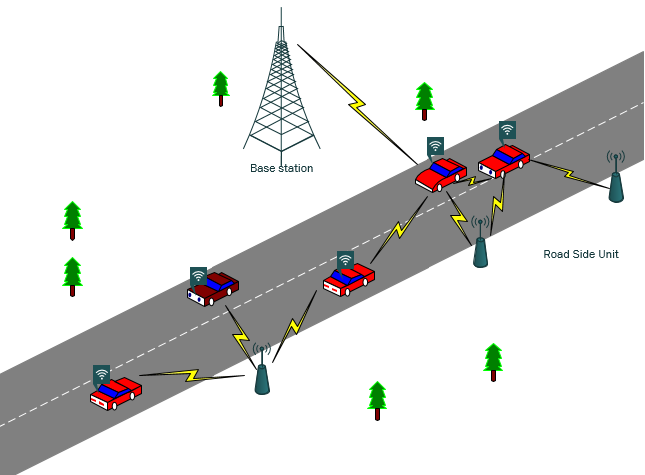
\includegraphics[width=0.9\textwidth]{fcw.png}
	\caption{Communication in a forward collision scenario}
	\label{fig}
\end{figure}
In communication scenario in Figure 3.2, we observe the farthest car on the right wanting to overtake the car that is in front of it. However, there’s another vehicle that is coming from the opposite direction and there’s a high chance that if the car is allowed to overtake, a collision might occur. This communication is relayed to all the other cars in the network through the Road side units. The car coming in the opposite direction will be made aware of the overtaking car, and a warning will be issued to the overtaking car to brake, or stay in its lane.

\subsubsection{Working of the algorithm}
 This algorithm for forward collision avoidance calculates the safe braking distance  $d_S$  as a function of speed and the GPS coordinates of the cars.
 
 From Newton's laws of motion:
 \begin{equation}
 	s = ut + \frac{1}{2} a t^2
\end{equation}

whereby $s$ is the distance covered by the leading vehicle, $u$ is its initial speed, $t$ is the time taken to cover the distance $s$, and $a$ is the acceleration of the leading vehicle. 
Assumption is that the leading vehicle is moving at a constant speed, hence acceleration $a$ = 0.
$time = \frac{distance}{speed}$ hence: 
Distance to Collision 

\begin{equation}
	DTC  = U_A \times \frac{-d_R}{U_r}
\end{equation} 

where $d_R$ is the range between the vehicles based on the Harvesine formula and $U_r$ is the relative velocity between the two cars

\begin{equation}
	U_r = U_b - U_a
\end{equation}

where: $U_b$ is the speed of the leading vehicle and $U_a$ is the speed of the following vehicle
But this would not be practical since the cars will keep on accelerating as they move. Hence: 
From 
\begin{equation}
	v^2 = u^2 + 2as 
\end{equation}
and
\begin{equation}
	v= u + at
\end{equation}

\begin{equation}
	t = \frac{U_r + \surd U_r^2 + 2as^2}{a_{l_v}}
\end{equation}

where ${a_{l_v}}$ is the acceleration of the leading vehicle
The equation for $t$ above the time to collision. Hence the distance to collision $DTC$ can be calculated from;

\begin{equation}
	DTC = \frac{U_r + \surd U_r^2 + 2as^2}{a_{l_v}} \times U_a
\end{equation}

There are three levels of thresholds defined for the warning distances and they take into account the parameters:
\begin{itemize}
	\item Speed
	\item Acceleration
	\item Distance between the vehicles, DTC
\end{itemize}

For whichever speeds or distances at any point in time, warnings will be triggered when the DTC is less than the three thresholds.

\subsubsection{Threshold 1}
From ------------------------------ equation 3.4 
\begin{equation}
	s = 0.5 \left[ \frac{v^2}{a} - \frac{u^2}{a}\right]
\end{equation}

But Distance = Speed $\times$ time, hence
\begin{equation}
	Distance = t_d \times U_a
\end{equation}

\[s = 0.5 \left[ \frac{v^2}{a} - \frac{u^2}{a}\right] + t_d \times U_a + D_o\]

\begin{equation}
	{D_{w1}} = 0.5 \left[ \frac{v^2}{a_{fv}} - \frac{u^2}{a_{lv}}\right] + t_d \times U_a + D_o 
\end{equation}

Where: $v$ is the final speed of the following vehicle and $u$ is the initial speed of the following vehicle. $a_{fv}$ is the acceleration of the leading vehicle, $a_{lv}$ is the acceleration of the following vehicle, $t_d$ is the delay time or brake time, $U_a$ is the speed of car A and $D_o$ is the distance between the following vehicle when/ if they stop.

\subsubsection{Threshold 2}
\begin{equation}
	{D_{w2}} = \frac{U_a^2}{19.6 \left[ \frac{a_{f_v}}{g} + f + G \right]} + t_d {V_{f_v}} + D_o
\end{equation}


Where: $g$ is the acceleration due to gravity, $G$ is universal gravitational constant, $Do$ is the distance between the following vehicle when/ if they stop. 
$f$ is the frictional coefficient based on the speed and it is provided by the range of values.


\begin{table}[H]
	\caption{Range of values for the frictional coefficient $f$ based on the speed} % title of Table
	\centering % used for centering table
	\begin{tabular}{| l | l |}
		\hline\hline
		$f$ & Values \\ \hline
		0.40 &  $U_a \textless 30$ \\ \hline
		0.38 &  $30 \textless Ua \textless 40$ \\ \hline
		0.37 &  $40 \textless Ua \textless 50$  \\ \hline	
		0.36 & 	$50 \textless Ua \textless 60$\\ \hline		
		0.35 & 	$Ua \textgreater 69$\\ \hline
	\end{tabular}
	%\label{tab:parameters-sleep-mode} 
\end{table}
	 
This warning is used to inform a driver that there is a vehicle in the same lane. If the actual vehicle spacing drops below this threshold, then the distance-to-collision is less than the total distance travelled by the vehicle during the delay time $t_d$ then the third threshold warning distance will be activated.


\subsubsection{Threshold 3}
From 
\begin{equation}
	s = ut + o.5at^2
\end{equation}

\begin{equation}
	{D_{w3}} = U_a t_d - 0.5{a_{lv}} t_d^2 + D_o
\end{equation}
where $a_{lv}$ is the acceleration of the leading vehicle, $t_d$ is the delay time or brake time, $U_a$ is the speed of car A and $D_o$ is the distance between the following vehicle when/ if they stop.


This threshold warning warns the driver to urgently take a decision to avoid collision immediately. If the driver doesn’t respond, the autonomous vehicle brakes or changes lane (if there is no incoming car in the opposite direction)

At every incoming basic safety message (threshold warning), the algorithm checks the difference between the DTC and the warning distances ($D_{w1}$, $D_{w2}$, and $D_{w3}$) then calculates the time interval to reach the warning distance considering the current speed.

In summary: 
\begin{itemize}
	\item The algorithm starts.
	\item The three distance warnings to be calculated are going to make use of the various input values obtained from the messages exchanged in the network. Basing on the values that it has been provided, it will issue either of the three appropriate warning signals: $D_{w1}$, $D_{w2}$, and $D_{w3}$.
	\item  If the time to warning ($t_{w1}$) is less than the GPS update period $t_{GPS}$, the first warning "Slow down vehicle on same lane" is issued to the appropriate vehicle. If not, the algorithm proceeds. 
	\item If the time to warning ($t_{w2}$) is less that $t_{GPS}$, the second warning "Brake or change lanes of there is no incoming car!" is issued to the appropriate vehicle.
	\item If the time to warning ($t_{w3}$) is less than the GPS update period, an urgent warning will be issued to the vehicle to brake or change lanes immediately.
	\item The algorithm ends.
\end{itemize}
   

%\begin{figure}[!h]

\tikzstyle{startstop} = [rectangle, rounded corners, text centered, text width=4cm, draw=red]
\tikzstyle{process} = [rectangle, text centered, draw=orange,  text width=8cm, ]
\tikzstyle{decision} = [diamond, text centered, draw=green,]
\tikzstyle{io} = [trapezium, trapezium left angle=70, trapezium right angle=110, text width=5cm, text centered, draw=blue]
\tikzstyle{arrow} = [thick,->,>=stealth]


\begin{tikzpicture}[node distance=4.5cm]
	
	\node (start) [startstop] { Start
	};
	\node (process) [process, below of=start] { 
		\[ D_{w1} = 0.5\left[ \frac{U_a^2}{a_{fv}} - \frac{U_b^2}{a_{lv}} \right] + \left( t_d \times U_a \right) + D_o \] 
		\[ D_{w2} = \frac{U_a^2}{19.6 \left[ \frac{a_{fv}}{g}  + f + G \right]} +t_d \times V_f + D_o \]
		\[ D_{w3} = U_a \times t_d - 0.5 \times a_{lv} \times t_d^2 + D_o\]
	};
	\node (io) [io, right of=process, xshift=3cm] {Inputs; $t_{GPS}$, $DTC$, $U_b$, $U_a$, $a_{fv}$, $a_{lv}$, $t_d$, $D_o$
	};
	\node (decision) [decision, below of=process] {Is $t_{w1}$ \textless  $t_{GPS}$?
	};
	\node (io2) [io, right of=decision, xshift=3cm] {Disp $t_{w1}$
		Disp (“Slow down, vehicle on same lane!”)
	};
	\node (decision2) [decision, below of=decision] { Is $t_{w2}$ \textless $t_{GPS}$?
	};
	\node (io3) [io, right of=decision2, xshift=3cm] {Disp $t_{w2}$
		Disp (“Second warning! Brake or Change Lanes if there is no incoming car!”)
	};
	\node (decision3) [decision, below of=decision2] { Is $t_{w3}$ \textless $t_{GPS}$?
	};
	\node (io4) [io, right of=decision3, xshift=3cm] {Disp $t_{w3}$
		Disp ("URGENT!! Brake or Change Lanes NOW!”)
	};
	\node (stop) [startstop, below of=decision3] { End
	};
	\draw [arrow] (start) -- (process);
	\draw [arrow] (process) -- (decision);
	\draw [arrow] (decision) -- node[anchor=east] {no} (decision2);
	\draw [arrow] (decision2) -- node[anchor=east] {no} (decision3);
	\draw [arrow] (decision3) -- node[anchor=east] {no}(stop);
	\draw [arrow] (io) -- (process);
	\draw [arrow] (decision) -- node[anchor=south] {yes}(io2);
	\draw [arrow] (decision2) -- node[anchor=south] {yes}(io3);
	\draw [arrow] (decision3) -- node[anchor=south] {yes}(io4);
\end{tikzpicture}
%\caption{The flow chart algorithm for forward collision}
%\end{figure}


\section{Intersection Movement Assist (IMA)}

IMA warns the driver of a vehicle when it is not safe to enter an intersection due to a high probability of colliding with one or more vehicles at intersections both where a signal is present (a “controlled” intersection) and those where only a stop or yield-sign is present (an “uncontrolled” intersection). The figure below represents one possible IMA scenario.


\begin{figure}[!ht]
	\hfill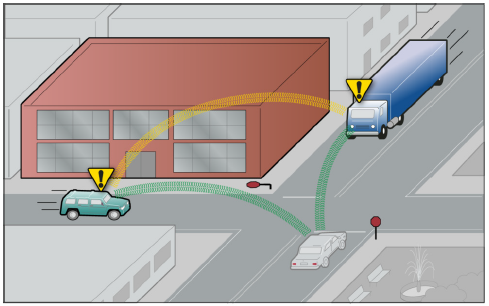
\includegraphics[width=0.7\textwidth]{wow.png}\hspace*{\fill}
	\caption{Two vehicles at potential risk of collision at intersection}
	\label{fig}
\end{figure}

In this scenario, the truck and the sports utility vehicle are at a risk of colliding because the drivers are unable to see each other approaching  the intersection and the stop sign is probably disabled. Both drivers would receive warnings of a potential collision, allowing them to take actions to avoid it.


\begin{figure}[!htbp]
	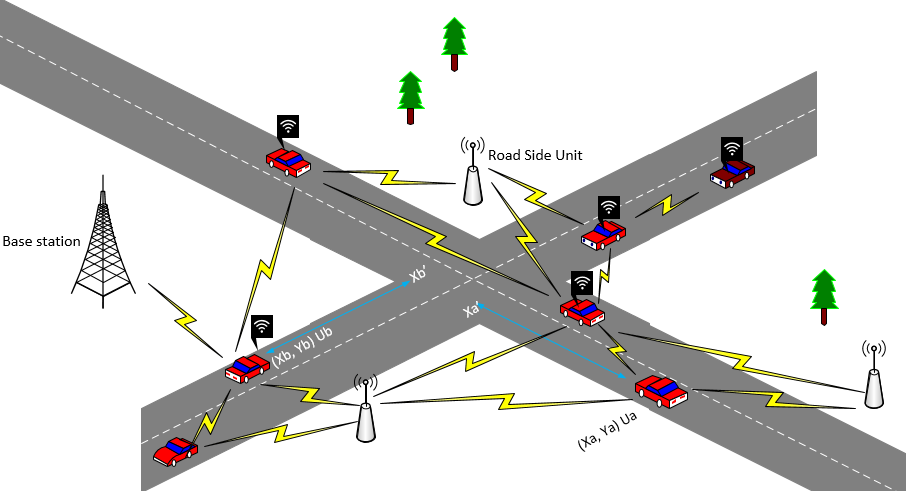
\includegraphics[width=0.95\textwidth]{IMA.png}
	\caption{Analysis of Intersection Movement Assist (IMA) with parameters}
	\label{fig}
\end{figure}

In the communication illustration of Figure 3.4, cars A and B (marked with coordinates) are approaching the junction and through the mesh network, all the cars are communicating. Without V2V, the two cars if over speeding, are bound to collide at the intersection. But with V2V, one of the cars is warned to slow down and let the car pass through the intersection first to avoid collision.

The GPS coordinates of Car B travelling at $U_b$ are ($X_b$, $Y_b$) as shown in Figure 3.4 while those for Car A travelling at speed Ua are ($X_a$, $Y_a$). After a certain time $t$, car B will have reached the intersection at coordinates ($X_b$', $Y_b$') and car will have reached at the coordinates ($X_a$', $Y_b$').

\subsubsection{Working of the algorithm}
\begin{itemize}
	\item The algorithm will take in the inputs as shared in the messages between the vehicles in the Vehicular Ad Hoc Network. 
	\item It will then calculate the time that each of the vehicles will take to reach the intersection. Time is calculated by $\frac{Distance}{Speed}$
	\begin{equation}
		t_A = \frac{X_a - X_a'}{U_a}
	\end{equation}
	\begin{equation}
		t_B = \frac{Y_a - Y_b'}{U_b}
	\end{equation}
	where $t_A$ is time taken for car A to reach the intersection, $t_B$ is the time taken for car B to reach the intersection B. 
	\item The algorithm then determines if the vehicles will reach the intersection at almost the same time (leaving a maximum allowable threshold value $t_h$). If the vehicles will successfully pass the intersection within allowable time interval of each other, then no warning signals are not issued.
	\item But if the algorithm determines that the time is less than the threshold, then it will calculate the final velocities $V_a$ and $V_b$ for each of the cars A and B, to which they should decelerate before they reach the intersection.
	 They are calculated from: 
	\begin{equation}
		V_A = \frac{X_a - X_a'}{t_A - t_h}
	\end{equation}
	\begin{equation}
		V_B = \frac{Y_b - Y_b'}{t_B - t_h}
	\end{equation}
	where $t_h$ is the threshold time below which it is not safe to continue travelling the same speed towards the intersection.
	\item The algorithm issues the warnings with the recommended speed values to either or both of the cars to decelerate. Car takes action to avoid collision by slowing down.
	\item The algorithm ends.
\end{itemize}

	
\tikzstyle{startstop} = [rectangle, rounded corners, text centered, text width=4cm, draw=red]
\tikzstyle{process} = [rectangle, text centered, draw=orange,  text width=4cm, minimum height=1cm ]
\tikzstyle{decision} = [diamond, text centered, draw=green, text width=3cm, minimum width=4cm]
\tikzstyle{io} = [trapezium, trapezium left angle=70, trapezium right angle=110, text width=4cm, text centered, draw=blue]
\tikzstyle{arrow} = [thick,->,>=stealth]

%\begin{figure}
\begin{tikzpicture} [node distance=4.5cm]
	\node (start) [startstop] {Start};
	\node (process) [process, below of=start] { Time to reach Intersection
		\[ t_A = \frac{X_a - X_a'}{U_a}\]
		\[ t_B = \frac{Y_a - Y_b'}{U_b}\]};
	\node (io) [io, right of=process, xshift=3cm] {Inputs; $U_a$, $U_b$, $X_a$, $X_a$’, $Y_b$, $Y_b$’
	};
	\node (decision) [decision, below of=process] { is $t_A$ \textless $t_B$ + $t_h$? };
	\node (start2) [startstop, right of=decision, xshift=3cm] {Proceed with journey	};
	\node (process2) [process, below of=decision] { 
		\[ V_A = \frac{X_a - X_a'}{t_A - th}\]
		\[ V_B = \frac{Y_b - Y_b'}{t_B - th}\]
	};
	\node (process3) [process, below of=process2] { Decelerate Car A or Car B to Speed $V_a$ or $V_b$ respectively };
	\node (stop) [startstop, below of=process3] { End };
	
	\draw [arrow] (start) -- (process);
	\draw [arrow] (process) -- (decision);
	\draw [arrow] (io) -- (process);
	\draw [arrow] (decision) -- node[anchor=east] {yes} (process2);
	\draw [arrow] (decision) -- node[anchor=south] {no}(start2);
	\draw [arrow] (process2) -- (process3);
	\draw [arrow] (process3) -- (stop);
\end{tikzpicture}
%\caption{Algorithm for Intersection Movement Assist}
%\end{figure}





\section{Blind Spot Warning}

Consider a scenario where two vehicles are approaching the junction from opposite sides of the same road. The two drivers are unaware of each other due to the blind spot. The base station placed at the junction constantly communicates with the cars and vice versa.
Once the signals are picked up by the receptors in the vehicle, another control module (OBU) within the vehicle processes the received signal. The OBU picks up the response signal in real time, analyses it and basing on the results, makes the decision to reduce the speed of the vehicle.
So the vehicles are not able to see each other physically but through V2V, they are made aware of the presence of the other approaching.

\begin{figure}[!hb]
\begin{center}
	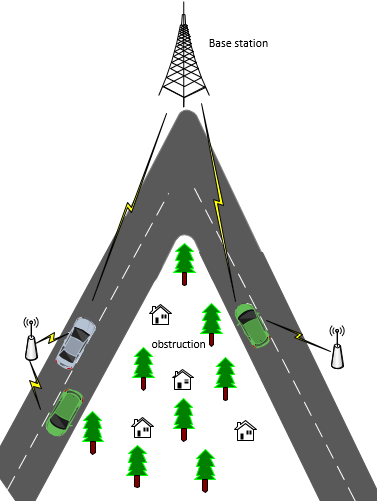
\includegraphics[width=0.6\textwidth]{blindspot.png}
	\caption{Analysis of blind spot}
	\label{fig}
\end{center}
\end{figure}

Either of the vehicles approaching the blind spot junction needs to decelerate at a value $–a$ = ? where $a$ is calculated from 
\begin{equation}
	v^2 = u^2 + 2as
\end{equation}
 
Let the threshold distance be $t_h$.
$u$ is be the speed of the car
$v$ is the maximum speed at which the car turns around the curve of a certain radius $r$.

From Force = Mass $\times$ acceleration
\[F_{friction} = \mu F_{normal}\]
\begin{equation}
	F_{gravity} = m \times g
\end{equation}
\[a_{centripetal} = \frac{v^2}{r}\]
\[ \mu F_{normal} = m \times \frac{v^2}{r} = \mu mg\]
\[ v^2 = \mu rg\]
\begin{equation}
	v = \surd\left( \mu rg\right)
\end{equation}
From \[v^2 = u^2 + 2as\]
\begin{equation}
	a = \frac{\surd\left( \mu rg\right) - u^2}{2s}
\end{equation}
where $a$ is the acceleration of the car, $u$ is the initial velocity of the car, $\mu$ is the coefficient of friction between the tyres and the road and it ranges between (0.1 - 0.4). 
One of the vehicles should decelerate at the value of above in order to round the corner at the final velocity $v$, to avoid collision.

\subsubsection{Working of the algorithm}
\begin{itemize}
	\item The algorithm starts.
	\item The algorithm determines if there are two cars each coming from the opposite direction. It does this with the help of their GPS coordinates (through the information exchanged in the VANET between the vehicles and the base station).
	\item If there are indeed two cars approaching the blind spot from both directions, the algorithm then determines if the distances at which they are at is less than the threshold td. If this is not the case, the cars proceed with their journey as before.
	\item If the distance is less than the threshold td, then the algorithm calculates the value of the deceleration and final velocity either or both of the vehicles should take on. 
	\item It then issues a warning signal to the vehicle to  decelerate to this value calculate in the last process box.
	\item The algorithm ends
\end{itemize}


\begin{tikzpicture} [node distance=4.5cm]
	\tikzset{startstop} = [rectangle, rounded corners, text centered, text width=4cm, draw=red]
	\tikzset{process} = [rectangle, text centered, draw=orange,  text width=4cm, minimum height=1cm ]
	\tikzset{decision} = [diamond, text centered, draw=green, text width=4cm]
	\tikzset{io} = [trapezium, trapezium left angle=70, trapezium right angle=110, text width=3cm, text centered, draw=blue]
	\tikzset{arrow} = [thick,->,>=stealth]
	
	\node (start) [startstop] {Start};
	\node (decision) [decision, below of=start] { Are two vehicles detected approaching the blind spot? };
	\node (io) [io, right of=decision, xshift=2cm] {Inputs: GPS coordinates $X_a$, $X_b$};
	
	\node (decision2) [decision, below of=decision, yshift=-2.5cm] { Is distance between vehicles and blind spot less than threshold distance td? };
	
	\node (start2) [startstop, right of=decision2, xshift=2.5cm] {Proceed with journey};
	
	\node (process) [process, below of=decision2, yshift=-1cm] { 
		\[v = \surd\left( \mu rg\right)\]
		\[a = \frac{\surd\left( \mu rg\right) - u^2}{2s}\]
		};
	
	\node (process2) [process, below of=process] { Warning; Slow vehicle down! Decelerate Vehicle A or B to deceleration value $a$.  };
	\node (stop) [startstop, below of=process2, yshift=1cm] { End };
	
	
	\draw [arrow] (start) -- (decision);
	\draw [arrow] (decision) -- node[anchor=east] {yes}(decision2);
	\draw [arrow] (io) -- (decision);
	\draw [arrow] (decision2) -- node[anchor=east] {yes}(process);
	\draw [arrow] (decision2) -- node [anchor=south] {no}(start2);
	\draw [arrow] (process) -- (process2);
	\draw [arrow] (process2) -- (stop);
	
	
\end{tikzpicture}


\section{The Communication Model}
The VANET is implemented using a 5G Cellular Network for it's high speeds and very low latency.

The cars will communicate with each other through wireless links (routers or On Board units) that are mounted on each vehicle / vehicular node. Each node within the Vehicular Ad hoc network acts as both the participant and the router of the network, as the nodes communicate through their intermediate nodes that lie within their transmission range. 
The VANET will have a range beyond which the vehicles will not be able to communicate
The On-Board Units, or OBUs that connect the vehicles to the 5G network will detect their positions and dynamic parameters using a GNSS (Global Navigation Satellite system) module. An in-vehicle tablet with a graphical interface can be placed inside the cars to enable information from the mobile router to be visualized. 

\subsection{The Role of the Base Stations}
Information are transmitted to every vehicle by the base stations (BSs) deployed along the road side. Two vehicles can communicate with one another directly as long as the Euclidean distance between two vehicles is less than the threshold value. 
Due to the mobility of vehicles, the topology of a VANET is changing over time, so the clusters of vehicles are splitting and merging over time, where a cluster is a maximal set of vehicles in which there is at least one hop between each pair of vehicles. Multi-hop communication allows a base station to only need to communicate to only one vehicle. Then by vehicle to vehicle communication, all vehicles in a cluster can receive or transmit messages.
The Base Station here acts as a controller that has the ability to make decisions for the vehicles given different scenarios. One of these scenarios could be if the collision avoidance decision that is made by a car in the VANET is probably not the best, it will decide a better option for the vehicle to take.

\subsection{The Role of the Road Side Units}
The road side units deployed along the road reinforce the mesh network by receiving the transmitted signals from the cars and retransmitting them. This is especially useful if the cars are too far away from each other and direct communication between them would be impossible. The road side units have no advanced functions and do not take part in any decision making processes in the network (like the autonomous cars and the base stations do).




\chapter{RESULTS AND ANALYSIS}

This chapter provides the results, their significance and how they were analyzed and manipulated to achieve the intended goals. 

\begin{table}[H]
\caption{Simulation Parameters for this project} % title of Table
\centering % used for centering table
    \begin{tabular}{| l | l |}
	 \hline\hline
    Parameters & Values \\ \hline
    Acceleration due to gravity &  $g = 9.8\,\text{m/s}^2$ \\ \hline
    Universal gravitational constant &  $G = 6.67408 \times 10^{-{1{1}}}\, \text{m}^3 \text{kg}^{-{1}} \text{s}^{-{2}}$ \\ \hline
	GPS update period &  $ t_{G_{P_{S}}} = 1\  \text{second}$  \\ \hline	
    Frictional Coefficient & $\mu = \left\{0.1, 0.4\right\}$\\\hline		
\end{tabular}
%\label{tab:parameters-sleep-mode} 
\end{table}

Figure 4.1: Simulation was done for a scenario whereby the speed of Car A ($U_a$) is less than the speed of Car B ($U_b$) and range $d_R$ is greater than safe distance $d_S$.
We observe Car A in (blue) accelerating from $40\,\text{m/s}^2$ until it reaches a safe distance behind Car B which is moving at $80\,\text{m/s}^2$. Once the safe distance has been reached, Car B then maintains a constant velocity at 80 together with the leading vehicle Car B

\begin{figure}[!ht]
	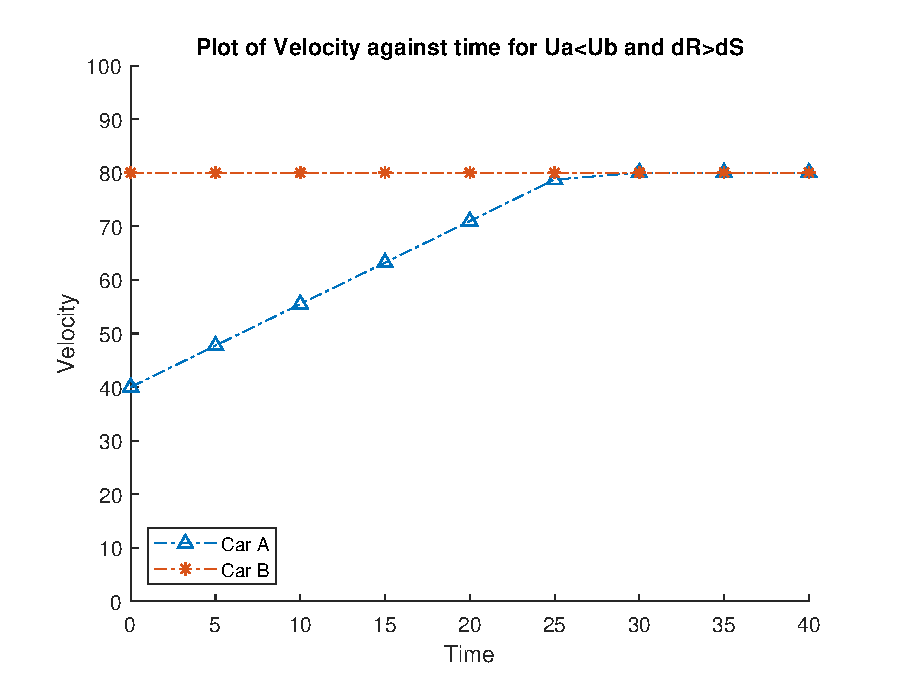
\includegraphics[width=0.9\textwidth]{acceleration.eps}
	\caption{When $U_a$ is less than $U_b$ and range $d_R$ is greater than safe distance $d_S$.}
	\label{fig}
\end{figure}

Figure 4.2: A similar simulation was done for a scenario whereby the speed of Car A ($U_a$) in red is greater than the speed of Car B ($U_b$) in blue and range $d_R$ is greater than safe distance $d_S$.
We observe Car A in (blue) decelerating from  $80\,\text{m/s}^2$ until it reaches a safe distance behind Car B which is moving at $40\,\text{m/s}^2$. Once the safe distance has been reached, Car B then maintains a constant velocity at $40\,\text{m/s}^2$ together with the leading vehicle Car B.

\begin{figure}[!hb]
	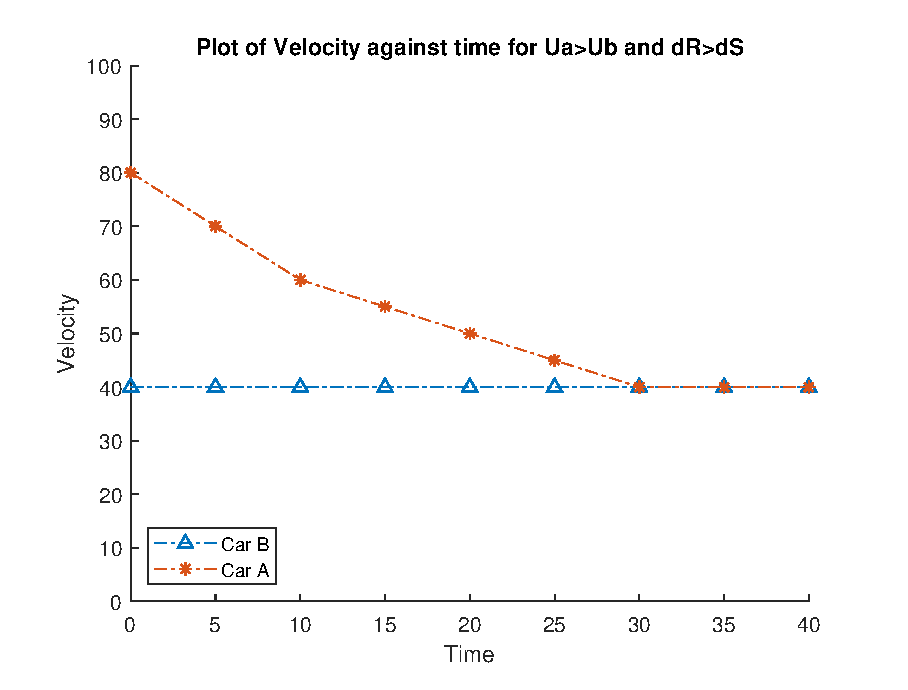
\includegraphics[width=0.9\textwidth]{deceleration.eps}
	\caption{When $U_a$ is greater than $U_b$ and range $d_R$ is greater than safe distance $d_S$.}
	\label{fig}
\end{figure}

Figure A.5: These were the results obtained when the algorithm was run in MATLAB. Certain data (from field) was fed in for the speed values; $U_b$, $U_a$ and GPS coordinates; $x_1$, $x_2$, $y_1$, and $y_2$. The algorithm hence produced the corresponding collision warning for the given values.
Running the algorithm with the values shown in the figure produced the collision warning "URGENT! Brake or Change Lanes Now!"
 
Figure A.6: Given values for speeds and GPS coordinates, the algorithm was run and it produced the result that indicated that the safe distance between the cars A and B was maintained.


% End with a conclusion chapter
\chapter{CONCLUSIONS}
%\label{chap:conclusion}

\section{Key Conclusions}
The algorithms for Blind spot and Intersection Movement Assist will ensure collision avoidance by signalling one of the cars to decrease (or rarely, increase) its speed as it approaches the blind spot junction. The rate of deceleration or acceleration will be determined by offsetting the time to collision by a certain threshold th in seconds.

The proposed forward collision avoidance algorithm will avoid collision either by braking at a safe distance behind the leading vehicle (if the range between the cars is greater than the safe distance) or by changing lanes and skipping the leading vehicle (if the safe distance between the cars has already been violated).

Forward Collision Warning applications using V2V technology can function in environments and under conditions beyond the current visual and radar detection systems (for example sunrise, sunset, rain, snow, or even any range greater than 300m), allowing for a more robust warning system. This can be attributed to the fact that the distances that would have to be covered by the transmission signals would be short, and hence leaving less chance for free space loss to occur. 

The Intersection Movement Assist algorithm can address a variety of crash types for real-world junction crossings. However, the analysis of this research has uncovered a number of limitations of the performance and test metrics used for the algorithm.
The current test procedures should thus be modified to reflect a greater range of speeds and variety of road geometry configurations, particularly non-perpendicular intersections, curved roads, and overpasses to allow for extended safety benefits. 


\section{Challenges}
Purchasing V2V equipment would have been very costly and the finances that we had to our disposal did not allow us to carry out a physical deployment of the collision avoidance models.

I recognize that additional refinement to the algorithms (as would be derived for the actual deployment of the models to actual vehicles) would be needed before minimum performance standards can be finalized.

\section{Recommendations}
The Government and Transport Ministry has the legal authority to mandate V2V (DSRC) devices in new light vehicles, and could also require them to be installed in commercial vehicles already in use on the road. The two powerful bodies also have the authority to mandate safety applications that are V2V-based, and to work with an outside entity (like the National Highway Traffic Systems Administration - NHTSA) to develop the security and communications infrastructures required to support deployment of V2V technologies in motor vehicles.

Even with the success of the algorithm simulations in MATLAB, in order to prove that V2V technology can work in a real-world environment on actual roads with regular drivers, additional items need to be in place beyond having the authority to implement a V2V system, in order for a potential V2V system to be successful. These items include:

\begin{itemize}
	\item A wireless spectrum: V2V communications transmit and receive messages at the 5.8-5.9 GHz frequency. The spectrum regulatory body should perhaps consider allowing “Unlicensed National Information Infrastructure” devices that provide short-range, high-speed, unlicensed wireless connections  to operate in the same area of the wireless spectrum as V2V. This could result in many more devices transmitting and receiving information on the same or similar frequencies, which could potentially interfere with V2V communications in ways harmful to its safety intent. More research needs to be done on whether these Wi-Fi enabled devices can share the spectrum successfully with V2V, and if so, how .
	
	\item V2V device certification issues: Auto manufacturers (and V2V device manufacturers), attempting to comply with a potential V2V mandate, could have a significant testing obligation to guarantee interoperability among their own devices and devices produced by other manufacturers. Entities providing the security systems should require that device manufacturers comply with interoperability certification requirements to ensure the reliability of the message content.
	
	\item Standing up security and communications systems to support V2V: In order to function safely, a V2V system needs security and communications infrastructure to enable and ensure the trustworthiness of communication between vehicles. The source of each message needs to be trusted and needs to be protected from outside interference.
	
	\item Privacy: The system should not collect or store any data identifying individuals or their vehicles, nor should it enable the government to do so. There should be no data in the safety messages exchanged that could be used by law enforcement or private entities to personally identify a speeding or erratic driver. Private entities should not be able to enable tracking through space and time of vehicles linked to specific owners or drivers.
	
	\item Consumer acceptance: If consumers do not accept this safety technology, then it will not create the safety benefits that it is expected to. One critical issue with consumer acceptance is maintenance. If the security system is designed to require consumers to obtain new security certificates or perhaps purchase additional expensive equipment, consumers might find the requirements too onerous.
\end{itemize}


\section{Ideas for Future Work}

Various aspects of Vehicle to Vehicle technology still need further investigation to support the transition from a prototype-level to a deployment-level system. Further research to move toward deployment can be conducted in the following areas.
\begin{itemize}
	\item Development of performance requirements for DSRC devices, as would be installed in both autonomous and non autonomous vehicles.
	\item Incorporation of GPS positioning advancements to improve V2V relative positioning; If two cars are aware of their GPS co-ordinates, comparison would allow the two to position each other, perhaps, ahead of time.
	\item Remedies to address false positive warnings from V2V safety applications. 
	\item Driver-vehicle interface performance to enhance crash avoidance warning effectiveness
	\item An appraisal of consumer acceptance of the technology. Before deployment, extensive research ought to be done to determine how the acceptable the technology will be to the general public.
	\item Evaluation of privacy risks that come with the implementation of a V2V communication system.
	\item An assessment of the security system to ensure a trusted and a safe V2V system. To determine which systems would provide maximal security and the requirements for implementations of such systems.
\end{itemize}


%\bibliographystyle{alpha}

\bibliographystyle{IEEEtran}


\begin{thebibliography}{1}
	
	\bibitem{traffic}
	T. W. H. Organisation, “Road Traffic Injuries," World Health Organisation, 7 February 2020. [Online]. Available: https://www.who.int/news-room/fact-sheets/detail/road-traffic-injuries. [Accessed 6th December 2020].
	
	\bibitem{systematic}
	 W. H. Organisation, “Systematic Reviews," World Health Organisation, July 2016. [Online]. Available: https://www.who.int/bulletin/volumes/94/7/15-163121/en/. [Accessed 5th December 2020].
	
	\bibitem{road}
	U. Nations, “Road Safety Performance Review Uganda," February, Geneva, 2018.
	
	\bibitem{talk}
	T. R. n. team, “If Only Our Cars Could Talk, What Would They Say?," 30 November 2017. [Online]. Available: https://www.danielrrosen.com/v2v-technology-advances-of-2017/. [Accessed 4 December 2020].
	
	\bibitem{vanet}
	P. B. a. V. Jindal, “Research Gate," September 2014. [Online]. Available: https://www.researchgate.net/publication/266148960 [Accessed 4 September 2020].
	
	\bibitem{dual}
	Mohamed Yousef; Ahmed Hosny; Wessam Gamil; Mohamed Adel; Hazem M. Fahmy; M. Saeed Darweesh; Hassan Mostafa, “Dual-Mode Forward Collision Avoidance Algorithm Based on Vehicle-to-Vehicle (V2V) Communication," IEEE, Windsor, Canada, 2018.
	
	\bibitem{protocols}
	Luca Delgrossi and Tao Zhang, Vehicle Safety Communications - Protocols, security and privacy, Canada: John Wiley and Sons, Inc., Hoboken, New Jersey, 2012. 
	
	\bibitem{qualcomm}
	Qualcomm, “Qualcomm," Qualcomm, 2020. [Online]. Available: https://www.qualcomm.com/invention/5g/what-is-5g: [Accessed 4 December 2020].
	
	\bibitem{readiness}
	Harding, J., Powell, G., R., Yoon, R., Fikentscher, J., Doyle, C., Sade, D., Lukuc, M., Simons, J., and Wang, J., “Vehicle-to-Vehicle Communications: Readiness of V2V Technology for Application," National Highway Traffic Systems Administration, 2014.
	
	\bibitem{fikasalama}
	Adminspeed, “Supporting Policy Engagement for Evidance Based Solutions," 01 April 2019. [Online]. Available: http://speed.musph.ac.ug/fika-salama-results/. [Accessed 7 December 2020].
	
	\bibitem{matlab}
	Mathworks, “MATLAB - Mathworks - MATLAB and SIMULINK," Mathworks Inc, [Online]. Available: https://www.mathworks.com/products/matlab.html. [Accessed 9 February 2020].
	
	
\end{thebibliography}


%% the bibliography style determines the format  in which both citations and references are printed,
%% other possible values are plain and abbrv
%%
%% If you want more control of the format of your citations you might want to take a look at
%% natbib.sty, which should be part of any standard LaTeX installation
%%
%% University regulations simply require that your citation style be consistent, so see what style
%% your supervisor recommends.

% Appendices start here



\appendix

\chapter{Appendix}

\begin{figure}[!ht]
	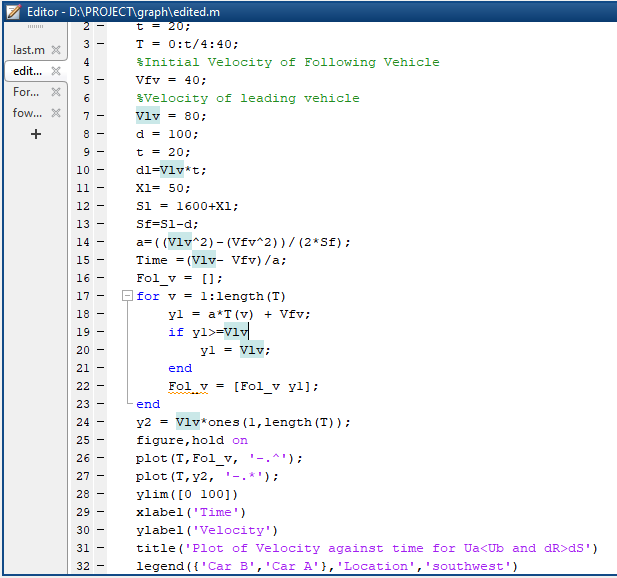
\includegraphics[width=0.9\textwidth]{accelerationcode.png}
	\caption{The code used to generate acceleration scenario in Fig 4.1.}
	\label{fig}
\end{figure}
\begin{figure}[!ht]
	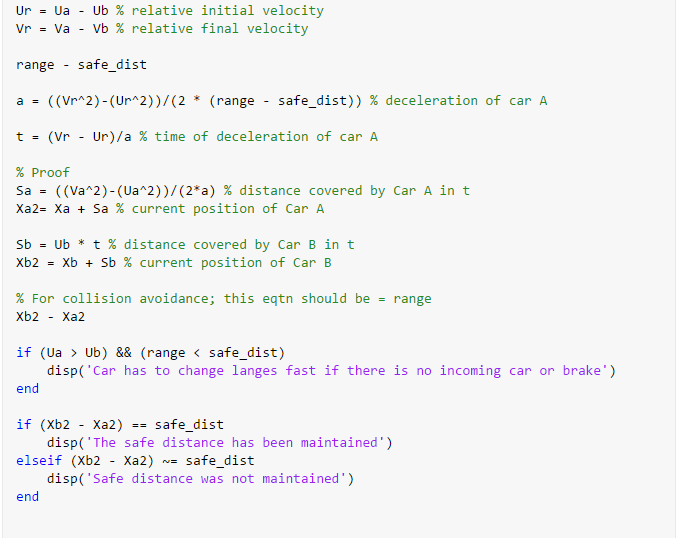
\includegraphics[width=1.0\textwidth]{pretty.png}
	\caption{The code used to determine if the safe distances between the cars in the forward collision scenario were maintained}
	\label{fig}
\end{figure}
\begin{figure}[!ht]
	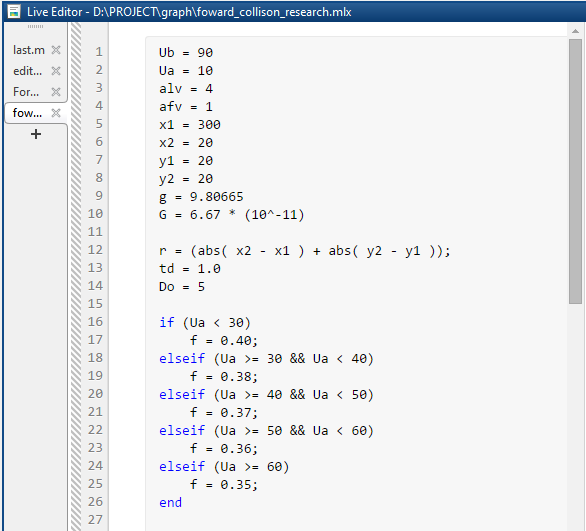
\includegraphics[width=0.8\textwidth]{xyz.png}
	\caption{Forward collision avoidance algorithm code - part 1 }
	\label{fig}
\end{figure}
\begin{figure}[!ht]
	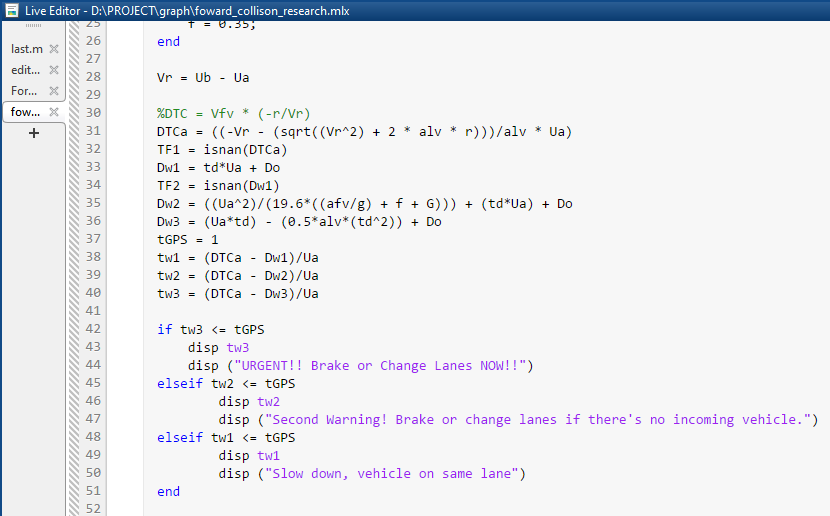
\includegraphics[width=0.9\textwidth]{xyz2.png}
	\caption{Forward collision avoidance algorithm code - part 2 }
	\label{fig}
\end{figure}

\begin{figure}[!htp]
	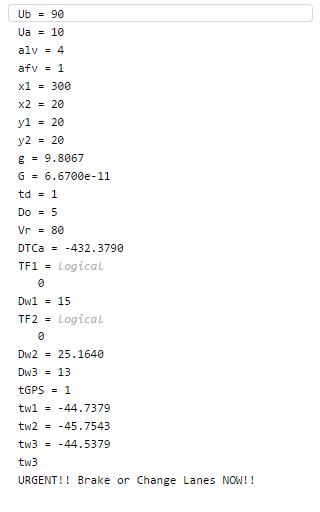
\includegraphics[width=0.55\textwidth]{Capture.png}
	\caption{Results obtained from running the forward collision avoidance algorithm}
	\label{fig}
\end{figure}

\begin{figure}[!htp]
	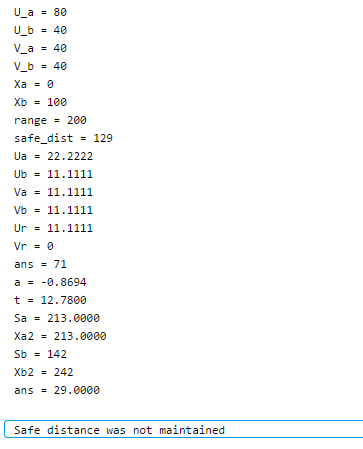
\includegraphics[width=0.6\textwidth]{safedistances.png}
	\caption{Results obtained from determining if safe distances were maintained}
	\label{fig}
\end{figure}


\end{document}
